\section{Simulation and optimization}
We use values derived from the literature to calibrate our models' fixed parameters. We simulate one model using a stepwise vaccination strategy and one model using s spline vaccination strategy.


\subsection{Calibration}
Within our model there  exist two vaccines $U_1$ and $U_2$. Whereas in the EU, as of July 2021, 4 vaccines have been approved and two are in the development phase \citep{ECa.2021}. To establish the link from our theoretical model to the real-world COVID-19 vaccines, we use data based on the four approved vaccines to calibrate our model. Vaccine $U_1$ represents the messenger ribonucleic acid (mRNA) vaccines and vaccine $U_2$ represent the vector vaccines. \\

Currently EU-approved mRNA vaccines are Comirnaty, also known as BNT162b2, from Pfizer-BioNTech as well as Spikevax, also known as mRNA-1273, from Moderna. The approved vector vaccines are Vaxzevria from Oxford-Astra Zeneca as well as Janssen, also known as Johnson \& Johnson COVID-19 vaccine, from Janssen Vaccines. \\
 
We use efficacy values reported within the literature to calibrate the vaccine-specific parameters $\delta_{k,l}$ and $\omega_{k,l}$. Efficacy describes the effect with respect to perfect conditions, whereas effectiveness measures the effect under real-world clinical settings \citep{Gartlehner.2006}. Therefore, real-world effectiveness could be lower than the numbers reported in Table \ref{tab:efficacy}. 
We use data from the early alpha virus type to calibrate the wild type parameters and data from the lately spreading delta variant to calibrate the mutant parameters.  In contrast to conventional vaccines, mRNA vaccines do not contain viral proteins themselves. They only contain the information human cells need to produce a virus trait that triggers the desired immune response \citep{Biontech.2021}. This new method has shown a significant improvement concerning immunity, yielding higher efficiacy values as can be seen in Table \ref{tab:efficacy}. 
{\renewcommand{\arraystretch}{1.4}
\begin{table}[h!]
\centering
\begin{center}
\scalebox{0.8}{
\begin{tabular}{lccp{10cm}}
\hline
\multicolumn{1}{l}{Vaccine} & \multicolumn{2}{c}{Efficacy} & \multicolumn{1}{c}{Sources}\\
\multicolumn{1}{l}{}&\multicolumn{1}{c}{alpha}&\multicolumn{1}{c}{delta}&\multicolumn{1}{c}{}\\
\hline
\rule{0pt}{2.6ex}Comirnaty & 94\%-95\% &  87\%-95\% &  \cite{Callaway.2021}, \cite{Nasreen.2021}, \cite{Polack.2020}, \cite{Prubeta.2021}, \cite{Sheikh.2021}\\
Spikevax & 94\% &  - & \cite{Oliver.2021}, \cite{Prubeta.2021} \\
Vaxzevria & 66\%-73\% &  60\%-71\% & \cite{Callaway.2021}, \cite{Emary.2021}, \cite{Prubeta.2021}, \cite{Stowe.2021}
 \\
Janssen &  66\% & - & \cite{Oliver.2021a}, \cite{Sadoff.2021} \\
\hline
\end{tabular}
}
\end{center}
\begin{tablenotes}
\scriptsize
\item Note: Efficacy is measured as protection against an infection after 14 days of the second vaccine shot. 
\end{tablenotes}
\caption{Vaccine efficacy}
\label{tab:efficacy}
\end{table}
}

Due to the recent spread of the delta variant, data is still limited and we did not find reliable sources for the delta efficacy of Spikevax and Janssen. For the latter, a recent study by \cite{Jongeneelen.2021} reports that even though real-world effectiveness has been shown, they found no efficacy for the Janssen vaccine against the delta variant. Since their study only included 8 individuals, we refrain from using the study to calibrate our model. \\

With respect to Table \ref{tab:efficacy}, we decided to set the protection of the mRNA vaccines against infection with the wild type (alpha variant) to be $\delta_{1, W} = 0.94$ and against infection with the mutant (delta variant) to be $\delta_{1, M} = 0.9$. For the vector vaccines we chose for the wild type $\delta_{2, W} = 0.7$ and for the mutant $\delta_{2, M} = 0.65$.\\

\cite{Abu.2021} report Comirnaty to protect from hospitalization by 97.4\%. \cite{Tenforde.2021} finds that Comirnaty and Spikevax yield 94\% protection against hospitalization within the age group of $\geq 65$ aged individuals. \cite{Voysey.2021} report a 100\% efficacy against hospitalization regarding Vaxzevria and the alpha variant. We generalize the empirical results and set the value against death protection $\omega_{k,l} = 0.99$ for all $k \in \{W,M\}$ and $l \in \{1,2\}$.\\

\cite{Harris.2021} found that in a study of more than 365,000 British households, mixed with vaccinated and unvaccinated individuals, that full vaccination with Comirnaty or Vaxzevria reduces the transmission probability by 40\%-60\%. We therefore set $\delta = 0.5$. \\

The basic reproduction number $R_l$ of virus type $l$ is the average number of unvaccinated individuals infected by one unvaccinated infectious individual. Translated to our model, this yields the following equations 
\begin{align}
R_W &= \frac{\beta}{\lambda} \\
R_M &= \frac{\eta \beta}{\lambda}, \notag
\end{align}
Recall that $1/\lambda$ is the average time an individual is infected and $\beta$, or $\eta \beta$, is the average number of individuals infected by one infectious individual per day. The German \cite{RKI.2021} reports the basic reproduction number to be between 2.8 and 3.8. Moreover, they state that an individual is infectious for about ten days infectious. We use $\lambda = 0.1, R_W = 3$ and $R_M = 3.6$, yielding $\beta = 0.3$ and $\eta = 1.2$. Note that these numbers do not take non-pharmaceutical measures such as testing and social distancing into account and therefore our simulated pandemic might have higher death numbers and be terminated earlier than the real-world COVID-19 pandemic. \\%We incorporate lower $R_l$ values within the sensitivity analysis to account for non-pharmaceutical policy measures against the pandemic. \\

\cite{Baud.2020} find a death rate of 5.7\% for symptomatic cases. However, this overestimates the true death rate due to undetected asymptomatic cases that did not result in death. \cite{Wu.2020} account for asymptomatic cases and find estimates to be between 2\%-3\%. We therefore use $p=2.5\%$ for our simulations.\\

To define the initial value problem, we set the initial population size of susceptible individuals in both countries to $y_0(X_S, C_A) = y_0(X_S, C_B) = 80$ million, a country size similar to Germany. Country A starts with ten wild type infectious individuals $y_0(X_I, C_A, V_W) = 10$ and country B with ten mutant type infected individuals $y_0(X_I, C_B, V_M) = 10$. We initially separate the virus types by country to examine the influence of heterogeneous virus infectiousness of appearing mutants across countries. All other compartments are set to zero at the beginning. \\

To specify the cross-border encounter modifier $b(d(A,B))$, we use tourism data from Germany and France. We use France since it is population-wise the largest country with a border to Germany. In 2016, $1,725,854$ individuals from France traveled to Germany and stayed for two days on average \citep{SBA.2017}. We divide this number by 366 to get an estimate of the average number of French individuals in Germany at each day in 2016 and scale it by $\frac{80}{67}$ to adjust that our second country has a population size of 80 million, whereas France has around 67 million inhabitants $\frac{2 \cdot 1,725,854}{366} \cdot \frac{80}{67
} \approx 11,261$. Assuming that the same number of French individuals have been in Germany every day and using equation \eqref{eq:prob_cross_border} with a constant proportion $\num(\neg X_D, C_B) / \num(\neg X_D) \approx y_0(\neg X_D, C_B) / y_0(\neg X_D) \quad \forall t \in [0,T]$, this yields 
\begin{align*}
b(d(A, B)) = \frac{11,261}{80,000,000} \approx 0.0002
\end{align*}
Note that this estimate is rather conservative since we do not take commuters and unregistered visits, such as shopping trips, into account. You find a section about the sensitivity of the model with respect to $b(d(A, B))$ within Appendix \ref{A:encounters}. \\

We set the length of the whole decision period to $T=140$ and subdivide the length of each decision interval $\mathcal{T}_i$ to 14 days. Even thoug we derive the model's parameters using days, we subsequently use weeks to label the axes to increase readability of the figures.

Figure \ref{fig:available_vaccine} depicts the inflow of both vaccines. The daily vaccine inflow $W_l(t)$ is computed using EU data of the vaccine inflow taken from the open-source data bank of the \cite{ECDC.2021}. The data reports the weekly inflow of vaccines for all countries within the EU. We accumulate the numbers of Corminarty and Spikevax to compute the total numbers of mRNA vaccines and accumulate the total numbers of Vaxzevria and Janssen to compute the total numbers of vector vaccines per week. We scale this number down to our model's population size by dividing it through the total number of EU habitants and multiplicate it by the number of individuals in our model. We subsequently accumulate the vaccines within each $14$-day interval $\mathcal{T}_i$ and divide this number by 14 to get the average number of vaccine doses inflow per vaccine and day. Thus, the inflow per day of each vaccine is constant within each interval $\mathcal{T}_i$ but varies across intervals and vaccines. As a results, we get the stepwise functions shown in Figure \ref{fig:available_vaccine}. 
\begin{figure}[h!]
\centering
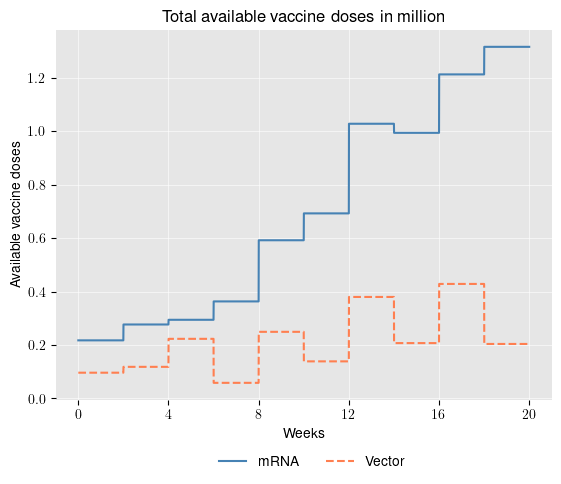
\includegraphics[scale=0.6]{images/available_vaccine.png}
\begin{flushleft}
\scriptsize{Note:} The total inflow of mRNA and vector vaccines is accumulated for each 2-week decision period and equally distributed across days. Real-world numbers are scaled down by a population size adjustment to account for the population size of our model.  
\end{flushleft}
\caption{Time course of exogenous vaccine inflow}
\label{fig:available_vaccine}
\end{figure}

Overall, the inflow increases over time. This is due to the improvement of manufacturer infrastructure over the time course of the pandemic in the real world and the constantly high demand for vaccines.


\subsection{Deterministic simulations}
We use Python and mainly its libraries libSBML \citep{Bornstein.2008} and AMICI \citep{Frohlich.2021} to implement our models. pyPESTO \citep{pyPESTO} is our main tool for optimization. To minimize the optimization problem, we use the L-BFGS-B algorithm \citep{Zhu.1997} for which pyPESTO uses Scipy's \citep{scipy.2020} implementation. For each optimization we run a muli-start using 50 starts and choose the corresponding vaccination strategy that minimizes the objective. We provide waterfall plots for the piecewise constant and the spline optimization within Appendix \ref{A:waterfall} in Figure \ref{fig:results_piecewise_waterfall} and Figure \ref{fig:results_splines_waterfall}. For each start, we draw uncorrelated start parameters $\theta_{l,i} \sim \mathcal{U}(0,1)$. In the case of Pareto optimal constraints, we only accept a starting vector $\Theta$ if the Pareto constraints $C.5$ and $C.6$ are satisfied. Otherwise, we reject it and draw a new sample until 50 starts are reached.\\

Piecewise constant and spline vaccination channels as functional forms of $f_l$ yielded very similar results regarding the trajectories of the compartments, which we see as enhancement of the robustness of our findings. However, we refrain from showing the same results twice and move the results from the piecewise constant approach to Appendix \ref{A:piecewise}.  \\

Figure \ref{fig:results_splines_numbers} provides a visualization of the number of deceased individuals using splines as functional form of $f_l$. We show the results for the current strategy (first row), the Pareto optimal strategy (second row), and the unrestricted strategy (third row) and split up the numbers of deceased individuals with respect to their country of origin. Both optimized strategies outperform the current strategy, which seems to be plausible given that the optimized strategies take the model states into account and the current strategy only follows a pre-allocation. The unrestricted strategy also outperforms the Pareto optimal strategy, which results from the nature of the optimization specification, since they are essentially the same optimization problem, but the Pareto parameter space is restricted by the two Pareto conditions $C.5$ and $C.6$. 
\begin{figure}[h!]
\centering
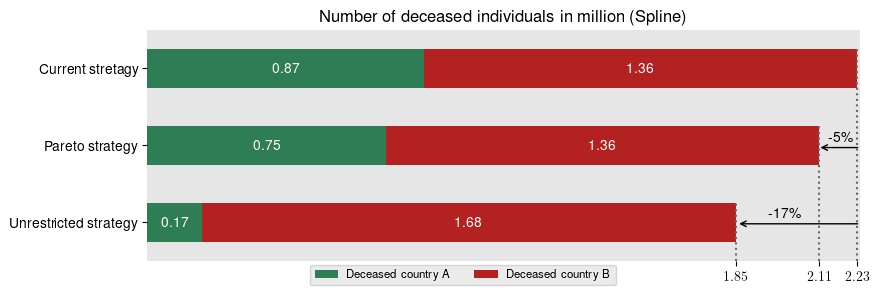
\includegraphics[scale=0.75]{images/splines_percentage_deviation.png}
\begin{flushleft}
\scriptsize{Note: The numbers within the boxes indicate the number of deceased individuals in millions with respect to the respective country and strategy. Numbers at the x-axis represent the total number of deceased individuals within one country. The percentage numbers indicate the change relative to the optimal strategy, e.g. $-5\%$ indicates that by implementing the Pareto strategy 5\% fewer individuals died in comparison to the current strategy.}
\end{flushleft}
\caption{Number of deceased individuals by country (splines)}
\label{fig:results_splines_numbers}
\end{figure}

The unrestricted strategy yields a reduction in deaths by around 17\% relative to the current strategy. However, given full knowledge of the outcome, policymakers in country B would not agree to implement this strategy due to the increase of around 320,000 deaths in country B. The Pareto strategy yields the same death cases in country B as the current strategy but at the same time, death cases in country A can be reduced by around 130,000, yielding an overall improvement of around 5\% relative to the current strategy. Thus, the Pareto optimal strategy is more likely to be approved by both countries given that it makes none of them worse but one country better off than the current strategy. \\

Figure \ref{fig:results_splines_allocation} depicts the vaccine inflow of each country dependent on the vaccination strategy. We show the results for the three strategies (columns) and split up the results by countries (rows). Due to equi-allocation, the vaccine inflow of the current strategy is 50\% of the total vaccine inflow shown in Figure \ref{fig:available_vaccine}. Most strikingly, the unrestricted strategy assigns vaccines to country B only between the 5th and the 9th week as well as at the first and the last periods. The period between the 5th and the 9th week is where the number of infectious cases increases exponentially within country B, as can be seen in Figure \ref{fig:results_splines_infectious_dead}.

The vaccine shortage in country B partly explains the large number of death cases in country B which we find in Figure \ref{fig:results_splines_numbers}. On the contrary, the Pareto strategy assigns much more doses to country B, especially at the end of the decision horizon. As seen in Figure \ref{fig:results_splines_numbers}, this comes with the cost of more deaths in country A compared to the unrestricted strategy but the benefit of an overall Pareto improvement compared to the current strategy.
\begin{figure}[h!]
\centering
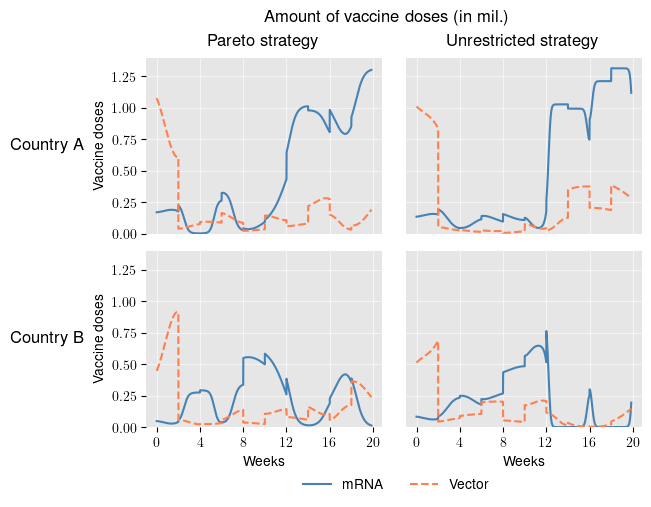
\includegraphics[scale=0.85]{images/splines_vaccine_total_quantity.png}
\begin{flushleft}
\scriptsize{Note:} Every column represents one vaccination strategy and every row represents one country. Both vaccines are indicated by the colors that are used throughout the paper. 
Every curve is the product of a piecewise constant vaccine inflow and a spline. Thus, the lines appear to be discontinuous piecewise polynomials. 
\end{flushleft}
\caption{Number of allocated vaccine doses (splines)}
\label{fig:results_splines_allocation}
\end{figure}

With respect to the current strategy, we observe that the optimized strategies are different from the current strategy. This is highlighted within Figure \ref{fig:results_splines_allocation_fractions} in Appendix \ref{A:fractions}, where we plot the course of the functions $f_l$. Figure \ref{fig:results_splines_allocation_fractions} also shows that the time courses of $f_1$ and $f_2$ show similar shapes indicating that vaccines are rather allocated as a bundle.\\
 
In Figure \ref{fig:results_splines_infectious_dead}, we trace out the trajectories of the number of infectious and deceased individuals according to the respective strategies (columns) and countries (rows). Regardless of the strategy, only the mutant spreads in country B. This is due to the initial allocation of ten mutant infected individuals in country B and ten wild type infected individuals in country A as well as the higher infectiousness of the mutant. The higher infectiousness of 20\% prevents the wild type from spreading in country B via cross-border infections. On the contrary, country A has to deal with both variants due to the cross-border infections. The unrestricted strategy can keep infections in country A below 2 million, whereas the Pareto strategy and the current strategy yield more than 7 million cases. 


\begin{figure}[h!]
\centering
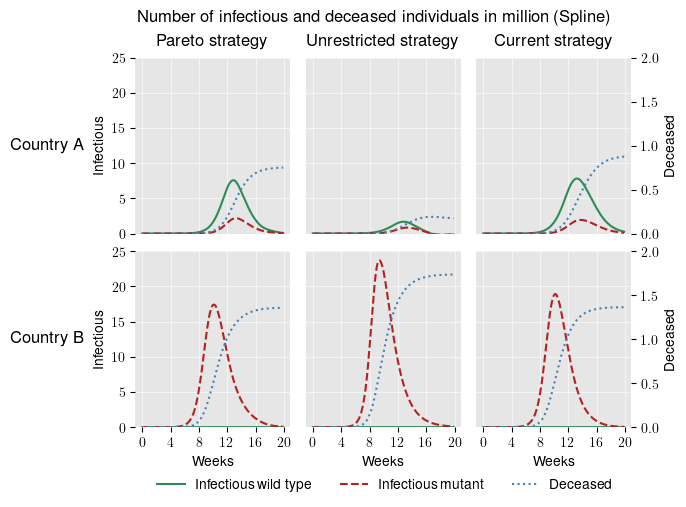
\includegraphics[scale=0.85]{images/splines_infectious_dead.png}
\begin{flushleft}
\scriptsize{Note:} Every column represents one vaccination strategy and every row represents one country. Every vaccine is indicated by its color that is used throughout the paper. The left y-axis is used for the number of infectious individuals (solid green and dashed red curves). The right y-axis corresponds to the number of deceased individuals (dotted blue line). Both viruses are associated with the color we have used throughout the paper. 
\end{flushleft}
\caption{Number of infectious individuals (splines)}
\label{fig:results_splines_infectious_dead}
\end{figure}



\clearpage
\subsection{Policy test with stochastic model}
We test the deterministically derived strategies within the stochastic set-up from Section \ref{sec:stochastic} to examine how they perform in an uncertain world where infections, recoveries, and deaths do not follow pre-determined patterns. We generate 500 samples per strategy by running Algorithm \ref{Algo:stochastic}. Unfortunately, we cannot simulate the algorithm with a set of random variables and test every strategy for this set and compare the results with a counterfactual interpretation. This is due to the nature of the problem the the means of the Poisson random variables in Equation \eqref{eq:tau_leaping} depend on the system's state and therefore the magnitude of randomness changes with the strategies, making counterfactual interpretations unfeasible.  \\ 

Figure \ref{fig:results_splines_stochastic_histogram} depicts the histograms of the number of deaths clustered by the three strategies. The average number of deceased individuals is between 0.78 and 0.95 million higher as in the respective deterministically derived strategies. However, we observe on average the same order as for the deterministic case. The unrestricted strategy yields the fewest deaths whereas most deaths are observed for the current strategy. 
\begin{figure}[h!]
\centering
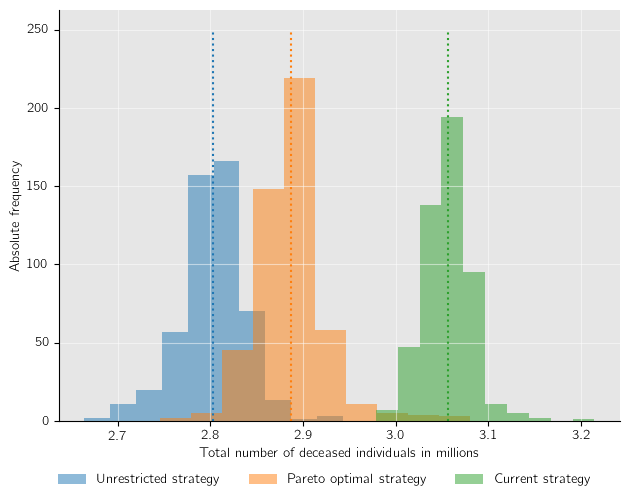
\includegraphics[scale=0.65]{images/splines_stochastic_histogram.png}
\begin{flushleft}
\scriptsize{Note:} Dotted lines are sample means. The total number of deceased individuals of a strategy is the sum of the respective number of deaths in country A and country B. We draw 500 samples per strategy. 
\end{flushleft}
\caption{Stochastically observed frequencies (splines)}
\label{fig:results_splines_stochastic_histogram}
\end{figure}
We plot the joint distribution of the deaths split up by country and the respective marginal histograms in Figure \ref{fig:histograms} in Appendix \ref{A:simulated_distr}.

In Figure \ref{fig:results_splines_infectious_dead_stochastic}, we explore how the number of infectious individuals varies within the samples. The course of infectious individuals of the unrestricted strategy in country B captures the deterministic numbers well. Within the other figures, the case numbers seem to be higher within the stochastic model, which is in line with the increased number of deaths observed in Figure \ref{fig:results_splines_stochastic_histogram}.

\begin{figure}[h!]
\centering
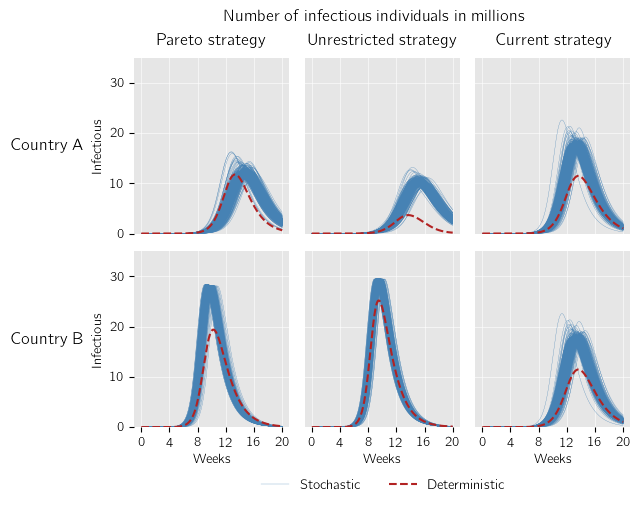
\includegraphics[scale=0.85]{images/splines_stochastic_infectious.png}
\begin{flushleft}
\scriptsize{Note:} Every column represents one vaccination strategy and every row represents one country. The thin blue lines depict all 500 simulations of the stochastic algorithm using the respective strategy. The dashed red depicts the respective infections within the deterministic model. 
\end{flushleft}
\caption{Number of infectious individuals using stochastic simulations (splines)}
\label{fig:results_splines_infectious_dead_stochastic}
\end{figure}















